\section{Results}
\begin{frame}
    \sectionpage
\end{frame}

\begin{frame}{Execution time}
    \begin{figure}
        \centering
        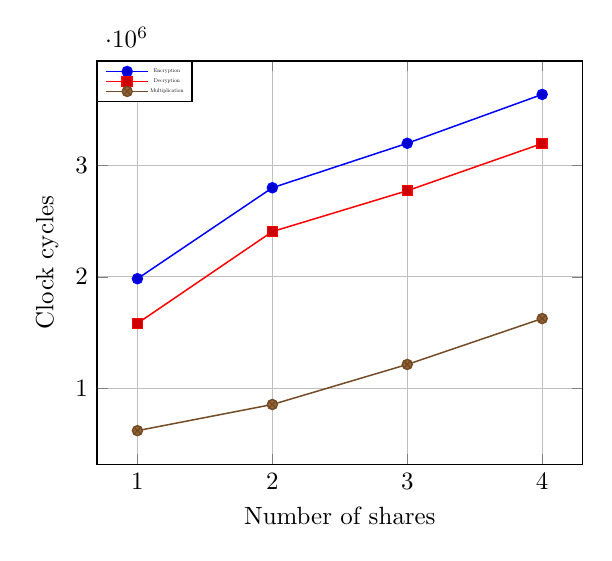
\begin{tikzpicture}[scale=0.9]
            \pgfplotsset{every axis/.append style={semithick}, legend style={at={(0,1)},anchor=north west, nodes={scale=0.6, transform shape}}}
    
        \begin{axis}[
            xlabel=Number of shares,
            ylabel=Clock cycles, 
            grid=major,
            xtick = {1,2,3,4}
            ]
        \addplot coordinates{
            (1, 1983894.79)
            (2, 2797433.27)
            (3, 3195107.26)
            (4, 3632298.13)
    
        };
        \addlegendentry{Encryption}
    
        \addplot coordinates{
            (1, 1584503.47)
            (2, 2405541.52)
            (3, 2770976.91)
            (4, 3193077.76)
    
        };
        \addlegendentry{Decryption}
    
        \addplot coordinates{
            (1, 624965.27)
            (2, 858842.66)
            (3, 1216993.20)
            (4, 1627512.25)
    
        };
        \addlegendentry{Multiplication}
        \end{axis}%
    \end{tikzpicture}%
    \end{figure}
\end{frame}

\begin{frame}{Execution time}
        \begin{figure}
        \centering
        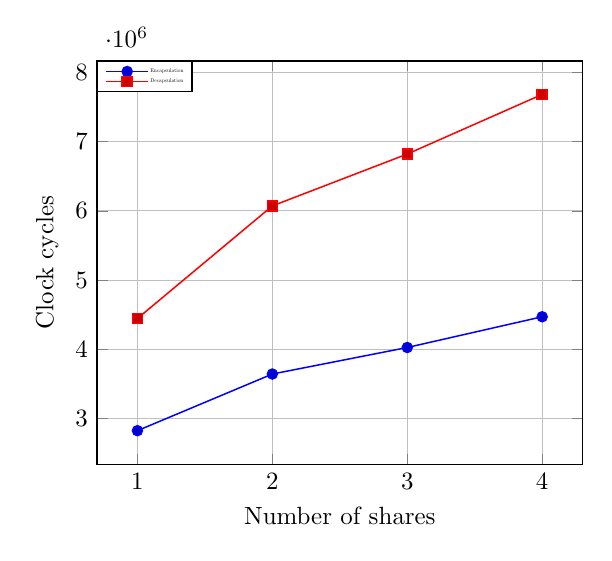
\begin{tikzpicture}[scale=0.9]
            \pgfplotsset{every axis/.append style={semithick}, legend style={at={(0,1)},anchor=north west, nodes={scale=0.6, transform shape}}}
        \begin{axis}[
            xlabel=Number of shares,
            ylabel=Clock cycles, 
            grid=major,
            xtick = {1,2,3,4}
            ]
        \addplot coordinates{
            (1, 2826067.47)
            (2, 3643555.40)
            (3, 4026514.86)
            (4, 4470225.81)
    
        };
        \addlegendentry{Encapsulation}
    
        \addplot coordinates{
            (1, 4445614.60)
            (2, 6070401.90)
            (3, 6819468.72)
            (4, 7680073.11)
    
        };
        \addlegendentry{Decapsulation}
        \end{axis}%
    \end{tikzpicture}%
    \end{figure}
\end{frame}

\begin{frame}{Performance loss}
    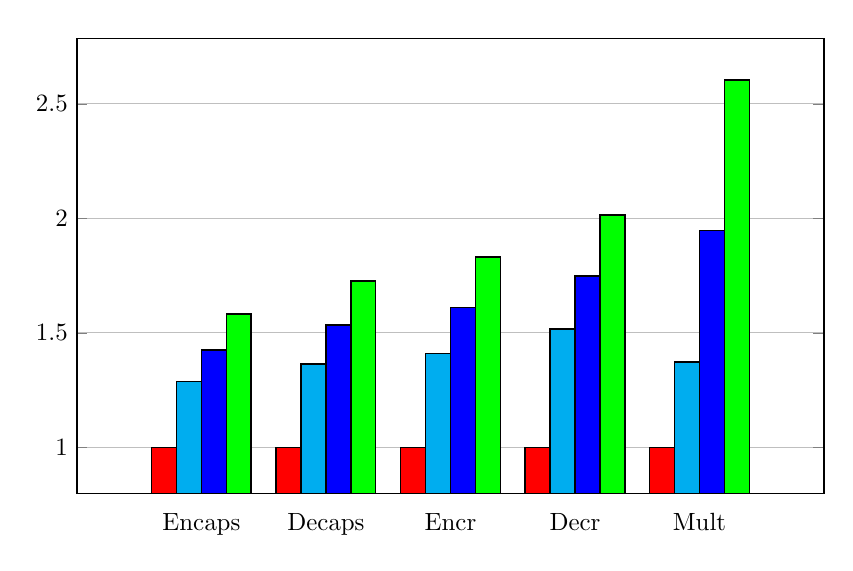
\begin{tikzpicture}[scale=0.9]
        \begin{axis}[
            width  = \linewidth,
            height = 8cm,
            major x tick style = transparent,
            %bar width=14pt,
            ymajorgrids = true,
            %ylabel = {Run time speed},
            ybar=0,
            symbolic x coords={Encaps, Decaps, Encr, Decr, Mult},
            xtick = data,
            scaled y ticks = true,
            enlarge x limits=0.25,
            ymin=0.8,
            legend cell align=left,
            legend style={
                    at={(1,1.05)},
                    anchor=south east,
                    column sep=1ex
            }
        ]
            % encaps
            \addplot[fill=red]
            coordinates {
                (Encaps, 1.0) 
                (Decaps,1.0) 
                (Encr,1.0)
                (Decr, 1.0)
                (Mult, 1.0)};
    
            \addplot[fill=cyan]
            coordinates {
                (Encaps, 1.2892) 
                (Decaps,1.3655) 
                (Encr,1.4100)
                (Decr, 1.5181)
                (Mult, 1.3742)};
            
            \addplot[fill=blue]
            coordinates {
                (Encaps, 1.4248) 
                (Decaps,1.5340) 
                (Encr,1.6105)
                (Decr, 1.7488)
                (Mult, 1.9473)};
    
            \addplot[fill=green]
            coordinates {
                (Encaps, 1.5818) 
                (Decaps,1.7276) 
                (Encr,1.8309)
                (Decr, 2.0151)
                (Mult, 2.6041)}; 
        \end{axis}
    \end{tikzpicture}
\end{frame}

\begin{frame}{Performance loss}
    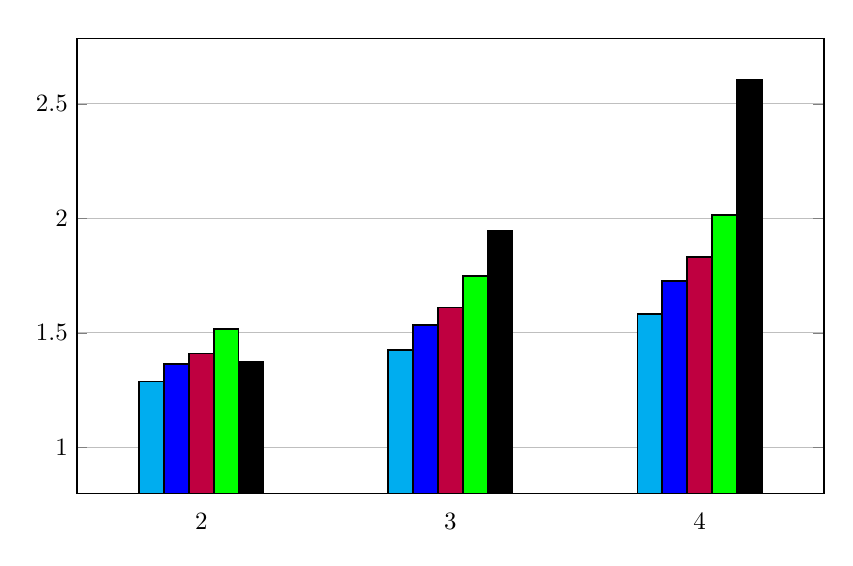
\begin{tikzpicture}[scale=0.9]
        \begin{axis}[
            width  = \linewidth,
            height = 8cm,
            major x tick style = transparent,
            %bar width=14pt,
            ymajorgrids = true,
            %ylabel = {Run time speed},
            ybar=0,
            symbolic x coords={2, 3, 4},
            xtick = data,
            scaled y ticks = true,
            enlarge x limits=0.25,
            ymin=0.8,
            legend cell align=left,
            legend style={
                    at={(1,1.05)},
                    anchor=south east,
                    column sep=1ex
            }
        ]
            % encaps
            \addplot[fill=cyan]
            coordinates {
                %(1, 1.0) 
                (2,1.2892) 
                (3, 1.4248)
                (4, 1.5818)
            };
    
            % decaps
            \addplot[fill=blue]
            coordinates {
                %(1, 1.0) 
                (2, 1.3655) 
                (3, 1.5340)
                (4, 1.7276) 
            };
                
            % encr
            \addplot[fill=purple]
            coordinates {
                %(1, 1.0)
                (2, 1.4100)
                (3, 1.6105)
                (4, 1.8309)
            };

            % decr
            \addplot[fill=green]
            coordinates {
                %(1, 1.0)
                (2, 1.5181)
                (3, 1.7488)
                (4, 2.0151)
            }; 
            
            % mult
            \addplot[fill=black]
            coordinates {
                %(1, 1.0)
                (2, 1.3742)
                (3, 1.9473)
                (4, 2.6041)
            };
        \end{axis}
    \end{tikzpicture}
\end{frame}

%\begin{frame}{Execution Time}
%    \begin{block}{Execution time (milliseconds)}
%        \begin{table}
%            \begin{tabular}{llllll}
%                \# & encaps & decaps & enc & dec & mul \\ \hline
%                1 & 201.86 & 317.54 & 141.71 & 113.18 & 44.64 \\
%                2 & 260.25 & 433.60 & 199.82 & 171.82 & 61.35 \\
%                3 & 287.61 & 487.10 & 228.22 & 197.93 & 86.93 \\
%                4 & 319.30 & 548.58 & 259.45 & 228.08 & 116.25             
%            \end{tabular}
%        \end{table}
%    \end{block}
%    \begin{block}{Percentual performance decrease}
%        \begin{table}
%            \begin{tabular}{llllll}
%                \# & encaps & decaps & enc & dec & mul \\ \hline
%                2 & 28.92 & 36.55 & 41.00 & 51.81 & 37.42 \\
%                3 & 42.48 & 53.40 & 61.05 & 74.88 & 94.73 \\
%                4 & 58.18 & 72.76 & 83.09 & 101.51 & 160.41
%            \end{tabular}
%        \end{table}
%    \end{block}
%\end{frame}

\begin{frame}{Constant-time execution}
    \begin{block}{Welch's t-test}
        Given two statistical populations $X_1$ and $X_2$ of $N_1$ and $N_2$ samples respectively:
        \begin{equation*}
            t = \frac{\bar{X_1} - \bar{X_2}}{\sqrt{\frac{s_{X_1}^2}{N_1} + \frac{s_{X_2}^2}{N_2}}}
        \end{equation*}\\
    Can be used to verify that the means of the distributions are equal (null hypothesis).\\
    Setting the confidence to 99.999\%, we accept $H_0$ for $|t| \leq 4.5$
    \end{block}
\end{frame}

\begin{frame}{Constant-time execution}
    \begin{block}{Test Vector Leakage Assessment}
        Based on the Welch's t-test, defines the two groups as:
        \begin{itemize}
            \item Random: use different inputs for each computation
            \item Fixed: use the same inputs for all computations
        \end{itemize}
        In case of random data (\textit{e.g.} masks), these are always generated randomly.
    \end{block}
\end{frame}

\begin{frame}{Constant-time execution}
    \begin{block}{Welch's t}
        \begin{table}
            \begin{tabular}{llllll}
                \# & encaps & decaps & enc & dec & mul \\ \hline
                1 & 0.94 & 4.57 & 25.66 & 10.26 & 30.09 \\
                2 & 6.00 & 3.36 & 4.62 & 5.96 & 4.96 \\
                3 & 0.29 & 1.69 & 1.60 & 5.88 & 3.51 \\
                4 & 0.13 & NA\footnote{Not enough memory} & 3.30 & 4.01 & 0.22
            \end{tabular}
        \end{table}        
    \end{block}
\end{frame}
